%--------------------------------------------------------------------------------------------------%
%   Version:    1.0
%   Last Mod:   20170307    
%         By:   Juan Medina juancamilomedina1989@gmail.com
%   Author:     Juan Medina juancamilomedina1989@gmail.com
%--------------------------------------------------------------------------------------------------%

%-------------------------------------------- PREAMBLE --------------------------------------------%
\documentclass[12pt]{report}
\usepackage[a4paper,width=150mm,headheight=110pt,top=25mm,bottom=25mm]{geometry}
\usepackage[utf8]{inputenc}
\usepackage{listings}
\usepackage{graphicx}
\usepackage{pgffor} 
\usepackage{xeCJK}
\usepackage{float}
\usepackage[utf8]{inputenc}
\usepackage[english]{babel}
\usepackage{multicol}
\usepackage{subfig}
\usepackage{subfigure}
\usepackage{subcaption}
\usepackage{graphics} 
\usepackage{fancyhdr}

\documentclass[a4paper,12pt]{book}
\usepackage[utf8]{inputenc}
\usepackage[english]{babel}
\usepackage{fancyhdr}
 
\pagestyle{fancy}
\fancyhf{}
\fancyhead[LE,RO]{\small Aurio Pinto}
\fancyhead[RE,LO]{\small Wireless Communication System}
\fancyfoot[CE,CO]{\small \leftmark}
\fancyfoot[LE,RO]{\small \thepage}
 
\renewcommand{\headrulewidth}{2pt}
\renewcommand{\footrulewidth}{1pt}
 
% \begin{document}
 
% \chapter{Using different page styles}
% \pagestyle{fancy}
% \fancyhf{}
% \rhead{Aurio Pinto}
% \lhead{Wireless Communication Systems}
% \fancyfoot[CE,CO]{\leftmark}
% % \fancyfoot[LE,RO]{\thepage}
% % \rfoot{\centering\thepage}

\graphicspath{{Images/}}

\usepackage[round, numbers,authoryear]{natbib}
\usepackage{color}
\usepackage[dvipsnames]{xcolor}

\definecolor{mycolor}{RGB}{30,75,180}
\definecolor{mycolor2}{RGB}{40,75,90}
% Lund colors
\definecolor{LUGreen}{RGB}{173,202,184}
\definecolor{LUPink}{RGB}{233,196,199}
\definecolor{LUBlue}{RGB}{0,0,128}
\definecolor{LUBronze}{RGB}{156,97,20}
\definecolor{LUblue}{RGB}{185,211,220}
\definecolor{LUGrey}{RGB}{77,76,68}

\usepackage[colorlinks = true,
            linkcolor = mycolor,
            urlcolor  = mycolor,
            citecolor = mycolor,
            anchorcolor = mycolor]{hyperref}

\usepackage[hypcap=true,font={small,it}]{caption}

\captionsetup{belowskip=2pt,aboveskip=2pt}
\bibliographystyle{abbrvnat}

\renewcommand{\chaptername}{}

\renewcommand{\figureautorefname}{figure} % lower case default ref
\renewcommand{\tableautorefname}{table} % lower case default ref
\newcommand{\latex}{\LaTeX\xspace}
\newcommand{\mcite}[1]{\textcolor{mycolor}{\citeauthor{#1} (\citeyear{#1})}}
\newcommand{\hcite}[1]{(\textcolor{mycolor}{\citeauthor{#1}, \citeyear{#1}})}
%----------------------------------------------------------------------------------------------------%

%--------------------------------------------- DOCUMENT ---------------------------------------------%
\begin{document}
%\fancyhead[RO,LE]{}

% Title page
    % \documentclass{ctexart}
\begin{titlepage}

\includegraphics{Images/tongji_university.jpg}\\
\vspace{2cm}
Final Report     in Wireless Communication Systems
    \begin{center}
        \vspace*{1cm}
        
        {\large \textbf{Will the World Improve with 5G Technology?}}
        
        \vspace{0.5cm}
       How Beneficial Can It Be?
        
        \vspace{1.5cm}
        by \\
        \vspace{1.5cm}
        Aurio Estefan Augusto Pinto \url{auriopinto2000@tongji.edu.cn}$
                
        \vspace{1.0cm}
    \end{center}

\noindent{
\textcolor{black}{{\bf Abstract} - 5G technology will not be an incremental advance on 4G. The previous four generations of cellular technology have each been a major paradigm shift that has broken backwards compatibility. And indeed, 5G will need to be a paradigm shift that includes very high carrier frequencies with massive bandwidths, extreme base station and device densities as well as unprecedented numbers of antennas. But unlike the previous four generations, it will also be highly integrative: tying any new 5G air interface and spectrum together with LTE and WiFi to provide universal high-rate coverage and a seamless user experience. To support this, the core network will also have to reach unprecedented levels of flexibility and intelligence, spectrum regulation will need to be rethought and improved, and energy and cost efficiency will become even more critical considerations. This research discusses all of these topics, identifying key challenges for future research and preliminary 5G standardization activities}}

\vfill
\textcolor[rgb]{0.5,0.5,0.5}{
    \begin{flushleft}
    { \small
    10052101 \\
    Sitifan - 1656038\\
    Professor: Yin Xuefeng \\
    % Examiner: [Full name] \\
    Word Count: 3000 \\
    }
    \end{flushleft}
}
      
\end{titlepage}


% Optional Chapters

    %\chapter*{Dedication}
    %\chapter*{Declaration}
    \chapter*{Acknowledgements}
    \textcolor{black}{I would like to express my great appreciation to Professor Yin Xuefeng, Vice Dean of the College of Electronic and Information Engineering for his consistent guidance and encouragement. I would like to thank him for his valuable feedback during his course on 5G technology.}\\
    
    \textcolor{black}{In addition, I wish to record my deep gratitude to a number of my classmates who have taken time out of their busy schedule to help translate a few sections of the course. As Mandarin is not my native language, my classmates continued to ensure I was able to work to my full potential without a language barrier.}\\
    
%   \textcolor{black}{Lastly I would like to thank my dear friend,  Zhu Dongzhe(Benzema) for his continued support throughout the whole project.}\\
   
   \textcolor{black}{Special thanks go to all the people who believed in me along the way.}
    

% Table of contents, list of figures, and list of tables
    {\hypersetup{linkcolor=black}
        \tableofcontents
        \listoffigures
        % \listoftables
    }
        {\hypersetup{linkcolor=mycolor}}
    
% Introduction
    \chapter{Introduction} 
    
\section{The Road to 5G}

\textcolor{black}{In only the past year, preliminary interest and discussions about a possible 5G standard have evolved into a full-fledged conversation that has captured the attention and imagination of researchers and engineers around the world. As the long-term evolution (LTE) system embodying 4G has now been deployed and is reaching maturity, where only incremental improvements and small amounts of new spectrum can be expected, it is natural for researchers to ponder “what’s next?”. However, this is not a mere intellectual exercise. Thanks mainly to the annual visual network index (VNI) reports released by Cisco, we have quantitative evidence that the wireless data explosion is real and will continue. Driven largely by smart phones, tablets, and video streaming, the most recent (Feb. 2014) VNI report and forecast makes plain that an incremental approach will not come close to meeting the demands that networks will face by 2020. In just a decade, the amount of IP data handled by wireless networks will have increased by well over a factor of 100: from under 3 exabytes in 2010 to over 190 exabytes by 2018, on pace to exceed 500 exabytes by 2020. This deluge of data has been driven chiefly by video thus far, but new unforeseen applications can reasonably be expected to materialize by 2020. In addition to the sheer volume of data, the number of devices and the data rates will continue to grow exponentially. The number of devices could reach the tens or even hundreds of billions by the time 5G comes to fruition, due to many new applications beyond personal communications. It is our duty as engineers to meet these intense demands via innovative new technologies that are smart and efficient yet grounded in reality. Academia is engaging in large collaborative projects such as METIS and 5GNOW, while the industry is driving preliminary 5G standardization activities.}

\section{Engineering Requirements for 5G}

In order to more concretely understand the engineering challenges facing 5G, and to plan to meet the requirements, it is necessary to first identify the requirements for a 5G system. The following items are requirements in each key dimension, but it should be stressed that not all of these need to be satisfied simultaneously. Different applications will place different requirements on the performance, and peak requirements that will need to be satisfied in certain configurations are mentioned below. For example, very-high-rate applications such as streaming high-definition video may have relaxed latency and reliability requirements compared to driver less cars or public safety applications, where latency and reliability are paramount but lower data rates can be tolerated.
\begin{flushleft}1) Data Rate: The need to support the mobile data traffic explosion is unquestionably the main driver behind 5G. Data rate can be measured in several different ways, and there will be a 5G goal target for each such metric:\end{flushleft}
\begin{flushleft}a) Aggregate data rate refers to the total amount of data the network can serve, characterized in units of bits/s/area. The general consensus is that this quantity will need to increase by roughly 1000 times from 4G to 5G.\end{flushleft}
\begin{flushleft}b) Edge rate, or 5user can reasonably expect to receive when in range of the network, and so is an important metric and has a concrete engineering meaning. Goals for the 5G edge rate range from 100 Mbps (easily enough to support high-definition streaming) to as much as 1 Gbps. Meeting 100 Mbps for 95be is extraordinarily challenging, even with major technological advances. This requires about 100 times advance since current 4G systems have a typical 5the precise number varies quite widely depending on the load, cell size, and other factors.\end{flushleft}
\begin{flushleft}c) Peak rate is the best-case data rate that a user can hope to achieve under any conceivable network configuration. The peak rate is a marketing number, devoid of much meaning to engineers, but in any case, it will likely be in the range of tens of Gbps. Meeting the requirements in (a) and (b), which are about 1000 times and 100 times the current 4G technology, respectively, are part of the main focus of this research.\end{flushleft}
\begin{flushleft}2) Latency: Current 4G roundtrip latencies are in the order of about 15 ms and are based on the 1 ms subframe time with necessary overheads for resource allocation and access. Although this latency is sufficient for most current services, anticipated 5G applications include two-way gaming, novel cloud-based technologies such as those that may be touchscreen activated (the “tactile Internet”), and virtual and enhanced reality (e.g., Google glass or other wearable computing devices). As a result, 5G will need to be able to support a roundtrip latency of about 1 ms, an order of magnitude faster than 4G. In addition to shrinking down the subframe structure, such severe latency constraints may have important implications on design choices at several layers of the protocol stack and the core network.\end{flushleft}
\begin{flushleft}3) Energy and Cost: As we move to 5G, costs and energy consumption will, ideally, decrease, but at least they should not increase on a per-link basis. Since the per-link data rates being offered will be increasing by about 100 times, this means that the Joules per bit and cost per bit will need to fall by at least 100 times. In this research, we do not address energy and cost in a quantitative fashion, but we are intentionally advocating technological solutions that promise reasonable cost and power scaling. For example, mmWave spectrum should be 10 to 100 times cheaper per Hz than the 3G and 4G spectrum below 3 GHz. Similarly, small cells should be 10 to 100 times cheaper and more power-efficient than macrocells. A major cost consideration for 5G, even more so than in 4G due to the new BS densities and increased bandwidth, is the backhaul from the network edges into the core\end{flushleft}

% \section{Research Problem}
% Lorem ipsum dolor sit amet, consectetur adipiscing elit. Duis ut ipsum nec orci interdum sollicitudin ut eu nunc. Pellentesque ultricies eros in justo sagittis, eget blandit velit aliquet. Aenean ac lectus nibh. Quisque ac est pellentesque, ullamcorper sem sit amet, pharetra quam. Morbi ullamcorper placerat diam, sed tincidunt odio.

% \subsection{Chapter Subheading}
% Lorem ipsum dolor sit amet, consectetur adipiscing elit. Duis ut ipsum nec orci interdum sollicitudin ut eu nunc. Pellentesque ultricies eros in justo sagittis, eget blandit velit aliquet. Aenean ac lectus nibh. Quisque ac est pellentesque, ullamcorper sem sit amet, pharetra quam. Morbi ullamcorper placerat diam, sed tincidunt odio.

% \section{Aim and Scope}
% Lorem ipsum dolor sit amet, consectetur adipiscing elit. Duis ut ipsum nec orci interdum sollicitudin ut eu nunc. Pellentesque ultricies eros in justo sagittis, eget blandit velit aliquet. Aenean ac lectus nibh. Quisque ac est pellentesque, ullamcorper sem sit amet, pharetra quam. Morbi ullamcorper placerat diam, sed tincidunt odio.

% \section{Outline of the Thesis}
% Lorem ipsum dolor sit amet, consectetur adipiscing elit. Duis ut ipsum nec orci interdum sollicitudin ut eu nunc. Pellentesque ultricies eros in justo sagittis, eget blandit velit aliquet. Aenean ac lectus nibh. Quisque ac est pellentesque, ullamcorper sem sit amet, pharetra quam. Morbi ullamcorper placerat diam, sed tincidunt odio.

     
% Theory
    \chapter{A key technology towards 5G}
    \textcolor{black}{While previous generations of wireless networks were characterized by fixed radio parameters and spectrum blocks, 5G will allow utilization of any spectrum and any access technology for the best delivery of services.
\item Air-interface and RAN systems will need to be completely redesigned to accommodate a new mobile access paradigm of massive capacity, huge numbers of connections, and ultra-fast network speeds.
\item 5G will feature native support for new kinds of network deployments, including ultra-dense radio networking with self-backhauling, device- to-device communications, dynamic spectrum refarming and radio access infrastructure sharing.}\\

\section{Technologies}

% \subsection{Millimeter Waves}

\text{Every new generation of wireless network delivers faster speed and more functionality to our smart phones. 1G brought us the very first cell phones, 2G let us text for the first time, 3G brought us online, and 4G delivered the speed that we enjoy today. However, as more users come online, 4G networks have just about reached their limit at a time when users want even more data for their smart phones and devices. Now we are headed towards 5G, the next generation of wireless. 5G will be able to handle 1000 times more traffic than today’s networks and it will be up to 10 times faster than 4G LTE. Simply imagine downloading an HD movie in under a second, and then let your imagination run wild with what might be possible. 5G will be the foundation for virtual reality, autonomous driving, the internet of things, and things we cannot even imagine. What exactly is a 5G network? The truth is, experts cannot tell us what 5G actually is because they do not even know yet. Right now, there are a few brands already out there. This research will be considering five brand technologies emerging as a foundation of 5G.}\\

\begin{figure}
    \centering
    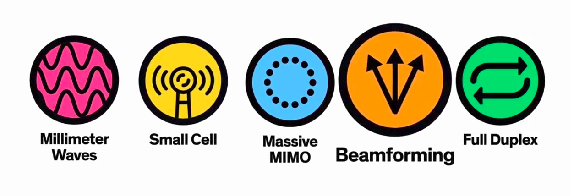
\includegraphics[width=10cm]{Images/now.png}
    \caption{Technologies}
    \label{fig:my_label}
\end{figure}

\subsection{Millimeter Waves}

\subsubsection{Introduction}

\text{{Studies on the fifth generation (5G) wireless communication system are gaining more momentum worldwide in an attempt to provide solutions for the exponential increase of mobile data traffic by 2020. Although 5G is in its embryonic stage, some trends have appeared on how to design 5G networks, such as to make it green and soft, as proposed by China Mobile. Multiple research topics have been identified as 5G candidates, including large-scale antenna systems (LSAS), non-orthogonal multiplex access, full duplex, spectrum sharing, high-frequency bands (e.g., millimeter-wave, mm Wave), high-density networks, new network architecture, new wave-form design, and so on. These technologies may have great potential in system performance improvement in 5G.}}\\

\subsection{Reference Signal Design}\\

\text{Smart phones and other electronic devices in your home use very specific frequencies on the radio frequency spectrum, typically those under 6 GHz but these frequencies are starting to get more crowded as carriers can only squeeze so many bits of data on the same amount of radio frequency spectrum. As more devices come online, we are going to start seeing slower service and more dropped connections. The solution is to open up some new real estage, so most of the companies such as Huawei are experimenting with broadcasting on shorter millimeter waves. Those that fall between 30 and 300 GHz of spectrum have never been used before for mobile devices and opening it up means more bandwidth for everyone. However, there is a catch: millimeter waves cannot travel well through buildings or other obstacles and tend to be absorbed by plants and rain. To avoid this problem, small cell networks can be used.}\\

\section{Small Cell}
Small cell networks: today’s wireless networks rely on tall high-powered cell towers to broadcast their signals over long distances, but we should keep in mind high-frequency millimeter waves have a harder time traveling through obstacles. This means that if we move behind an obstacle, we lose our signal. Small cell networks can solve this problem by using thousands of low-power mini base stations. These base stations would be much closer together than traditional towers, forming a sort of relay team to transmit signals around obstacles. This technology would be especially useful in cities, as the user moved behind an obstacle his smart phone would automatically switch to a new base station in better range of his device, allowing him to keep his connection.

\section{Full Duplex}
Full duplex: back in the day we used a wall gataki and in order for us to communicate using this technology, we had to take turns taking and listening. Today’s cellular base stations have that exact same hold-up as basic antennas can only do one job at a time either transmit or receive. This is because of a principle called reciprocity which is the decency for radio waves to travel both forward and backward along the same frequency. To understand this, it helps to think of waves like a train loaded up with data. The frequency is traveling on a train track, but if there is a second train trying to go in the opposite direction on the same track you are going to get some interference. Until now, the solution has been to have the trains take turns, or to put all the trains on different tracks or frequencies but this can be made a lot more efficient by working around reciprocity. Other researchers have used silicon transistors to create high speed switches that halt the backward role of these waves. It is like a signaling system that can momentarily reroute the trains so that they can get past each other. This means there is a lot more traffic on each track, and everything is a whole lot faster.
% MIMO most stands for multiple-input multiple-output, today’s 4G base stationshave about a dozen ports for antennas that handle all cellular traffic but massive MIMO base stations can support about a hundred ports this could increase the capacity of toda’s networks by a factor of 22 or more accurent with the experts massive MIMO comes with its own complications today’s cellular antennas broadcast information in every direction at once and all of those crossing signals could cause serious interference, which is one of the reason why 5G jumped the next tecnology above.\\

\section{Beam forming }
Beam forming is more precisely like a traffic signaling system for cellular signals instead of broadcasting in every direction. It would allow a base station to send a focus stream of data to a specific user. This precision prevents interferences and is way more efficient. This means stations could handle more incoming and outgoing data streams at once. In this research, it is explained how it works as well. If we are in a cluster building and you try to make a phone call, your signal is ricocheting off of surrounding buildings and crisscrossing with other signals from users in the area. A massive MIMO (multiple-inlet multiple-outlet, more on this is the next paragraph) base station receives all of these signals and keeps track of the timing and the direction of their arrival. It then uses signal processing algorithms to triangulate exactly where each signal is coming from and plots the best transmission route back through the air to each phone. Sometimes it will even bounce individual packets of data in different directions off of buildings or other objects to keep signals from interfering with each other, the result is a coherent data stream sent only to \\

\begin{figure}[t]
    \centering
    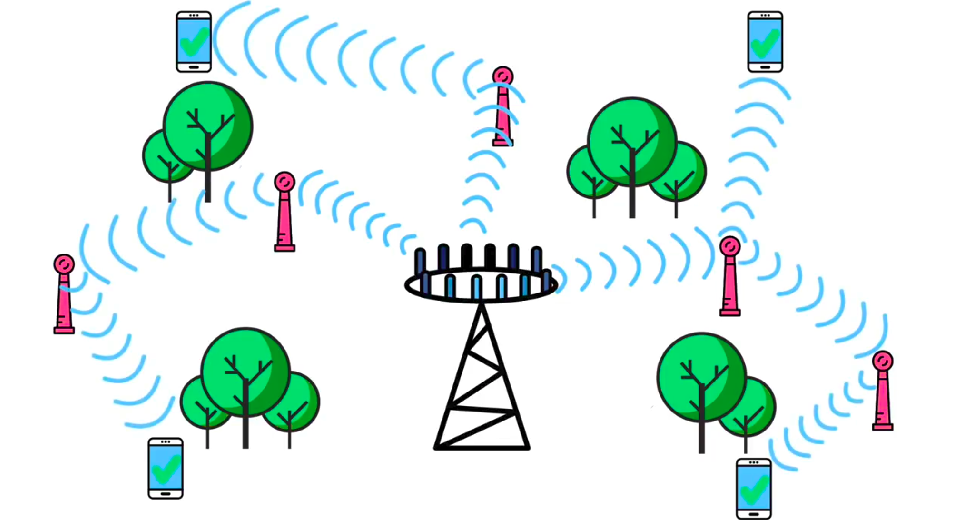
\includegraphics[width=9cm]{Images/small-cell.png}
    \caption{Small Cell}
    \label{fig:my_label}
\end{figure}

\begin{figure}
    \centering
    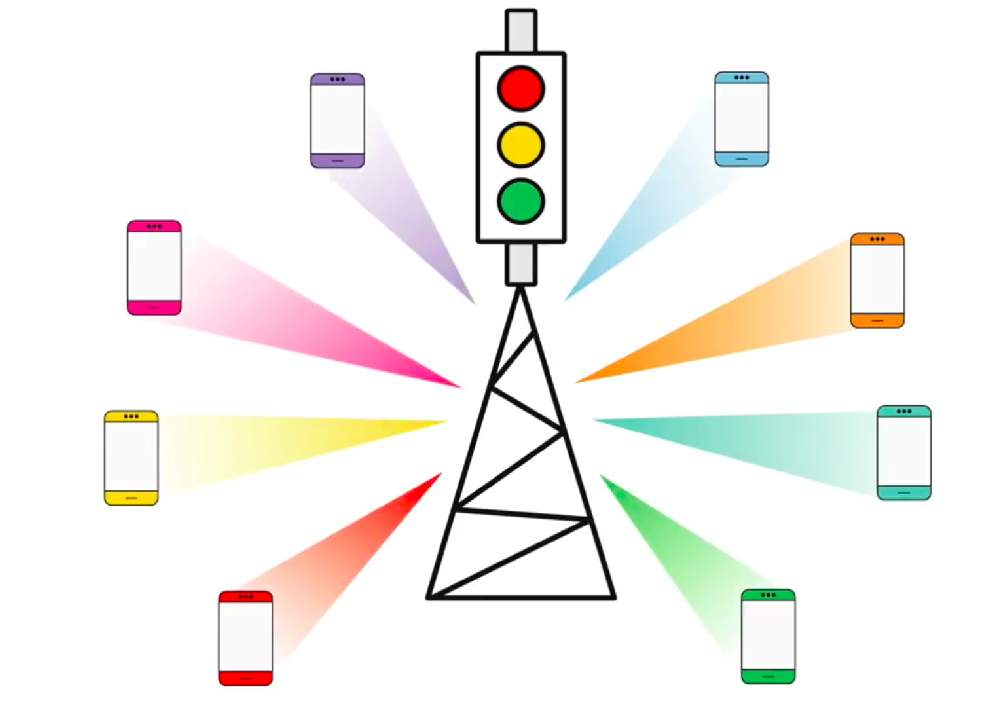
\includegraphics[width=8cm]{Images/Massive.png}
    \caption{Full-duplex}
    \label{fig:my_label}
\end{figure}\\

\section{Massive MIMO}
MIMO stands for Multiple-Input Multiple-Output. Today’s 4G base stations have about a dozen ports for antennas that handle all cellular traffic, but massive MIMO base stations can support about a hundred ports. This could increase the capacity of today’s networks by a factor of 22 or more. Currently, according to experts massive MIMO comes with its own complications. Today’s cellular antennas broadcast information in every direction at once and all of those crossing signals could cause serious interference, which is one of the reasons why 5G jumped to the next technology which will be discussed in further paragraphs..\\

    \figureautorefname
    
    
% Data
    \chapter{Perspective of Investment}
    \section{Smart Cities}
    \textcolor{black}{5G will provide the fundamental infrastructure for building smart cities, which will push mobile network performance and capability requirements to their extremes.
\item Low latency and extremely high reliability, however, will also be essential requirements for the likes of mobile industrial automation, vehicular connectivity, and other IoT applications. Applications like smart sensors and text-based messaging are examples of extremely high-volume applications that will require very low data rates and will not be sensitive to latency.}

% \begin{enumerate}
% \item	Reliability, which, for example, could depend on whether they are estimates or more direct evidence;
% \item	Representativity, which is about how typical the data are; for example, you may have arguments why the very few cases are typical or you may carry out statistical tests;
% \item Validity, which is about the relevance of the data for your case. Strictly speaking, sometimes no valid data are available but one may argue that there are other data which could be used as ‘proxies’.) 
% \end{enumerate}
}
\section{How 5G will enhance the finance industry}
From ATM machines to online and mobile banking, the financial services industry has often been an early adopter of digital technology.
\item According to research done by ATT and IDG, 81 percent of financial institutions have made technology changes at the corporate and/or branch level in recent years.
\item With mobile usage continuing to accelerate at a rapid pace, many customers are actively seeking new services to match the evolving technologies in their pockets and on their wrists. To meet these demands, banks must be more agile than ever.
5G technology is poised to help banks and other finance companies deliver the new, innovative mobile services consumers want.


% \section{Finance and BAT}
% Lorem ipsum dolor sit amet, consectetur adipiscing elit. Duis ut ipsum nec orci interdum sollicitudin ut eu nunc. Pellentesque ultricies eros in justo sagittis, eget blandit velit aliquet. Aenean ac lectus nibh. Quisque ac est pellentesque, ullamcorper sem sit amet, pharetra quam. Morbi ullamcorper placerat diam, sed tincidunt odio.

\section{Beyond customers}
5G’s benefits are expected to extend beyond customers. Financial professionals will also be able to use them to create more efficient back-end processes.
\item In insurance, damage appraisers could use 5G-enabled high-speed connectivity to send dozens of photos back to the head office quickly, without having to wait to reach their office or home network. Using this technology, insurance companies could serve customers more quickly and automatically, especially when combining claims adjustment processes with AI.
The future of financial services is mobile. As 5G enhancements create more reliable, responsive networks, they can help banks and other financial institutions ensure that this future is more productive, efficient and protected.


\subsection{Political Stage}
\subsubsection{America VS China}
When it comes to these two potential countries, it makes us wonder what exactly is 5G technology? And what is the deal with 5G? We might be tempted to think it is simply 4G but a little bit faster. In reality, it is a lot faster, so fast in fact that it can change the world as we have mentioned above briefly.
\item The new world of 5G technology promises to transform our lives by connecting millions of devices and enabling everything from driverless cars to smart homes. Up to 20 times faster than the 4G most of us use now, 5G’s lightning-fast technology will accelerate and interconnect everything
\item Downloading a two-hour film on 3G would take about 26 hours, on 4G you would be waiting six minutes, and on 5G you would be ready to watch the film in just over three and half seconds, what a world.
\item 5G is not only about download speeds, it is a game changer for everything. With 5G it is possible to have cities where everything is able to communicate. For example, doctors could perform surgeries from the other side of the world. Can you imagine a world where your videos never buffer, and your calls never drop?
\item There is no denying the technology is great. But. . . why do China and the U.S. care so much about who develops it?
\item The same reason they care about anything: there is a funny term “Benjamins” (i.e., money).
\item When the U.S. won the 4G race earlier this decade, it provided a nearly 100 billion boost to the gross domestic product. The stakes of the 5G race are even higher. If the U.S. wins, it will create an estimated three million jobs and add approximately 500 billion to GDP.
\item However, the fight over 5G is not just about money, and downloading films. No, it is also or mostly about power. If you control 5G access to everything people are doing online, you control everything.
\item Right now, the best 5G technology is made by the company Huawei. As this company is Chinese, many governments do not trust that the 5G will be secure.
\item Critics fear that allowing China to build 5G could enable the Chinese to spy on other countries or even to switch off the flow of data we will all depend on.
\item Imagine if Huawei becomes the leading 5G provider in the world, then China could spy on everyone, which is terrible for the U.S., because that is what the U.S. intends to do.
Those are the stakes: jobs, money and power.
\item While America is developing its own 5G, China’s 5G is so far ahead it will set the trends.
This is a race many people are saying the U.S. have already lost. Luckily, the U.S. have a maniac on their team who is willing to play dirty.
\item May 16: President Trump signed an executive order banning U.S. companies from using Telecom equipment deemed to be a national security threat. And that is a direct shot at China and tech giant Huawei.
\item Donald Trump could see the U.S. was not going to win, so he got a crowbar and pulled a Tonya Harding on China’s 5G.
\item Finally, President Trump cannot really be blamed for his actions, because how else can the U.S. win this race? Even if the U.S. do manage to cripple Huawei and China, it is not like the U.S. will suddenly have great 5G. You will not just have 5G overnight. Unless the U.S. pretends that it does.
\item It is a race that might be lost for the U.S., because this is considered the new space race. So maybe the U.S. can win this race the same way it won the last one (just fake it).

% \subsection{America VS China}

% \section{Huawei and ZTE}
    
% Methods
    \chapter{Cases for Potential Use of 5G}
    % \subsubsection{Imagining the mobile services of the next decade}
    \section{5G Ecosystem}
{As a leader in 5G technology, Huawei has completed inter-operability development testing (IODT) with mainstream chip, terminal, and network vendors. Huawei became the first company worldwide to launch the industry-first 5G commercial chip with 3GPP release 15. Huawei are the only vendor who can provide end-to end commercial solutions, vigorously promoting the maturity and commercial use of the 5G industry chain.}

\begin{figure}
    \centering
    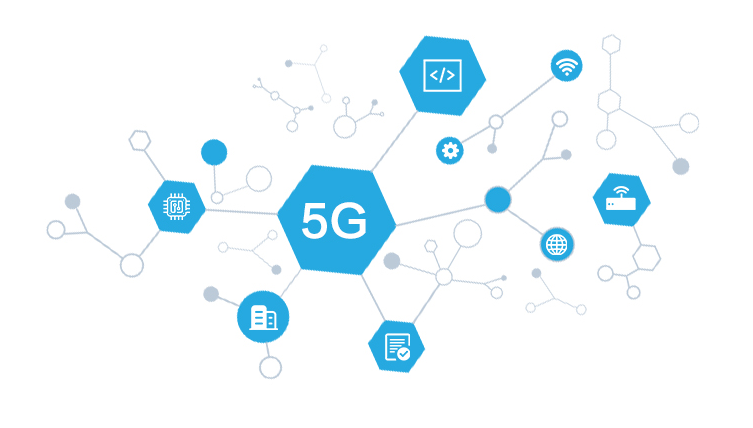
\includegraphics[width=11cm]{Images/lastimg.png}
    \caption{5G Ecosystem}
    \label{fig:my_label}
\end{figure}

\section{The Approach}
\subsubsection{Imagining the mobile services of the next decade.}

{As with each preceding generation, the rate of adoption of 5G and the ability of operators to monetize it will be a direct function of the new and unique use cases it unlocks. Thus, the key questions around 5G for operators are essentially\\ \item a. What could users do on a network which meets the 5G requirements listed above that is not currently possible on an already existing network?\\  \item b. How could these potential services be profitable?\\

\item These technologies have a number of potential use cases in both entertainment (e.g., gaming) and also more practical scenarios such as manufacturing or medicine and could extend to many wearable technologies. For example, an operation could be performed by a robot that is remotely controlled by a surgeon on the other side of the world. This type of application would require both high bandwidth and low latency beyond the capabilities of LTE, and therefore has the potential to be a key business model for 5G networks.\\ 

\item However, it should be pointed out that VR/AR systems are very much in their infancy and their development will be largely dependent on advances in a host of other technologies such as motion sensors and heads-up display (HUD). It remains to be seen whether these applications could become profitable businesses for operators in the future\\}

\subsubsection{Autonomous Driving/Connected Cars}

Enabling vehicles to communicate with the outside world could result in considerably more efficient and safer use of existing road infrastructure. If all of the vehicles on a road were connected to a network incorporating a traffic management system, they could potentially travel at much higher speeds and within greater proximity of each other without risk of accident - with fully-autonomous cars further reducing the potential for human error. While such systems would not require high bandwidth, providing data with a command-response time close to zero would be crucial for their safe operation, and thus such applications clearly require the 1 millisecond delay time provided in the 5G specification. In addition, a fully ‘driverless’ car would need to be driverless in all geographies, and hence would require full road network coverage with 100 percent reliability to be a viable proposition.

\subsubsection{Wireless Cloud-Based Office/Multi-Person Videoconferencing}

High bandwidth data networks have the potential to make the concept of a wireless cloud office a reality, with vast amounts of data storage capacity sufficient to make such systems ubiquitous. However, these applications are already in existence and their requirements are being met by existing 4G networks. While demand for cloud services will only increase, as now they will not require particularly low latencies and therefore can continue to be provided by current technologies or those already in development. While multi-person video calling - another potential business application - has a requirement for lower latency, this can likely be met by existing 4G technology.

\subsection{Machine-to-Machine Connectivity (M2M)}
M2M is already used in a vast range of applications but the possibilities for its usage are almost endless. Our forecasts predict that the number of cellular M2M connections worldwide will grow from 250 million this year to between 1 and 2 billion by 2020, dependent on the extent to which the industry and its regulators are able to establish the necessary frameworks to fully take advantage of the cellular M2M opportunity. Typical M2M applications can be found in ‘connected home’ systems (e.g., smart meters, smart thermostats, smoke detectors), vehicle telemetries systems (a field which overlaps with Connected Cars above), consumer electronics and health-care monitoring. Yet the vast majority of M2M systems transmit very low levels of data and the data transmitted is seldom time-critical. Many currently operate on 2G networks or can be integrated with the IP Multimedia Subsystem (IMS) – so at present the business case for M2M that can be attached to 5G is not immediately obvious.

\subsubsectionA True Requirement for a Generational Shift?}
Thus, many of the services that have been put forward as potential ‘killer apps’ for 5G do not require a generational shift in technology and could be provided via existing network technologies. Only applications that require at least one of the key 5G technical requirements –sub-1ms latency and Gbps downlink speed – can be considered true next generational business cases.\item Of these two requirements, reducing latency to sub-1ms levels may provide the greatest technical challenge. Meanwhile, operators are already making a considerable amount of progress in increasing the data speeds of their existing networks by adopting LTE-A \item technologies. While it is important to note that although many of the use cases and services discussed in this section do not strictly require 5G, they could offer an enhanced user experience on a 5G network. However, this amounts to an incremental benefit that is more difficult to market than a genuine new service, and not a core component of any 5G business case.

% \begin{figure}
%     \centering
%     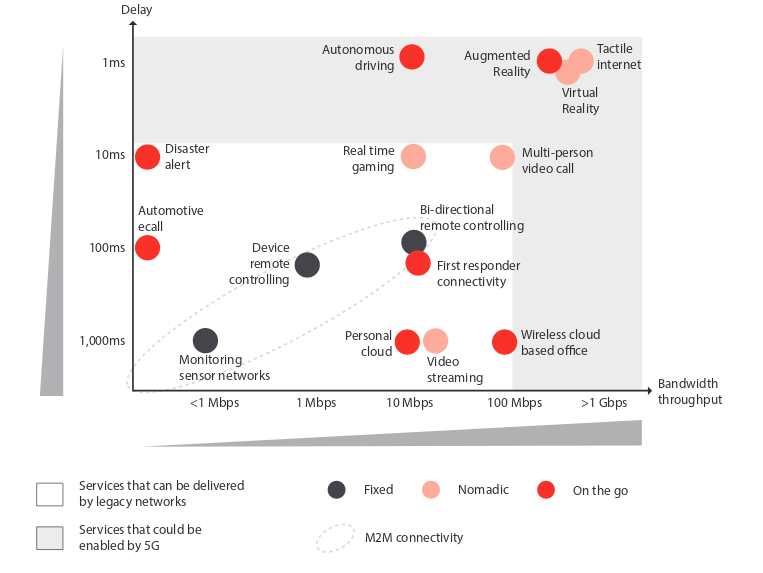
\includegraphics[width=6cm]{Images/prespective.png}
%     \caption{Caption}
%     \label{fig:my_label}
% \end{figure}
    
% Empirical Analysis
    \chapter{5 Empirical Analysis}
    \section{A Survey on 5G Network Technologies from a Social Perspective}
\textcolor{black}{The rapid advancement in communication technology innovations results in proliferation of heterogeneous smart devices in the network. The inter-communication of these devices is usually related to their social behavior and relationships. Furthermore, the upcoming 5G network promises to bind all the network technologies like Internet of Vehicles (IoV), Internet of Things (IoT), Mobile Cloud Computing (MCC), Smart Grids (SG), Big Data, and Device-to-Device (D2D) communications in a common network. To achieve this unified goal, one promising possibility is to exploit social properties of various smart devices used by these technologies. Exploitation of social aspect can dispense optimized networking while avoiding problems such as network congestion, resource allocations, and the like. It also leads to convergence of upcoming 5G network technologies and human society, giving rise to a new paradigm known as “socio-5G network technologies”. The state-of-the-art research on socio-5G network technologies is reviewed with the focus on six important technologies that 5G promises to support in one integrated network: IoV, IoT, MCC, SG, Big Data, and D2D communications. We also discuss the open issues related to combining social aspects with above-mentioned technologies.}
% \section{Results}
% Lorem ipsum dolor sit amet, consectetur adipiscing elit. Duis ut ipsum nec orci interdum sollicitudin ut eu nunc. Pellentesque 

% % \textcolor{red}{When placing tables (\autoref{tab:econ}) within the body of the text, the citation is placed above the table.} 

% \begin{figure}
%     \centering
%     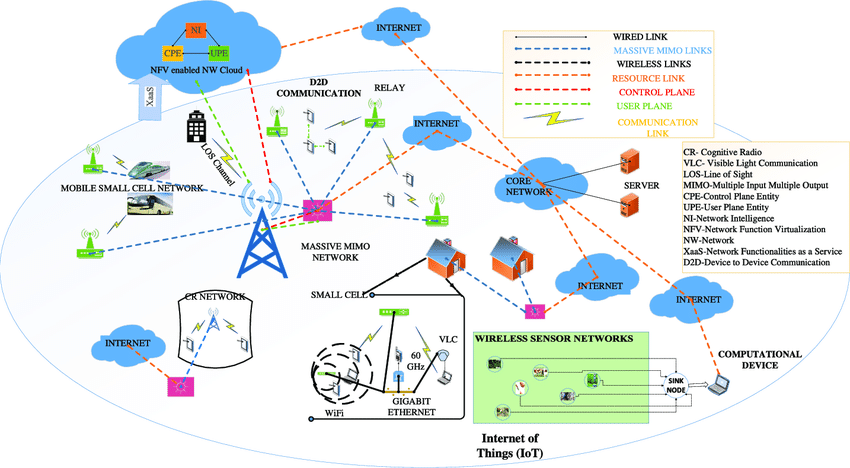
\includegraphics[width=17cm]{Images/result.png}
%     \caption{Result}
%     \label{fig:my_label}
% \end{figure}

% \begin{table}[!ht]
%   \centering
%   {\small {\it \caption{The economic argument \label{tab:econ} \hcite{econ}}}}
%   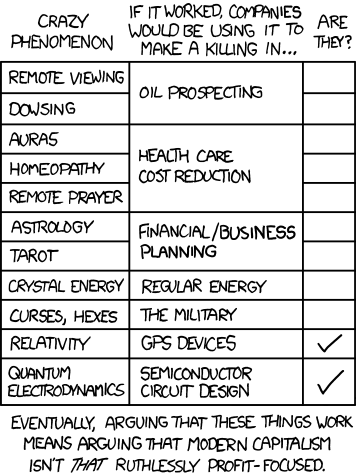
\includegraphics [scale=0.5]{Images/the_economic_argument.png} \\
% \end{table}

% \vfill

\newpage 

\section{Discussion}
\textbf{Sukhdeep Singh}Sukhdeep Singh completed his bachelor’s and master’s degree in technology from GyanVihar University, Jaipur, India. Currently, he is a PhD research scholar in the ECE Department of the College of Information and Communication Engineering, Sungkyunkwan University, South Korea. His research interests are mobile video streaming in social networks, cloud computing, and green networking. He has presented at five international conferences and has two journal publications.\item\textbf{Navrati Saxena}is an associate professor in the Electrical Engineering Department, Sungkyunkwan University, South Korea. She worked as an \item\textbf{Abhishek Roy}is currently working in the System Design Lab of Networks Systems Division, Samsung Electronics in South Korea. He received his PhD degree in 2010 from Sungkyunkwan University in the College of Information and Communication Engineering, MS degree in 2002 from the University of Texas at Arlington, USA, and BE degree in 2000 from Jadavpur University, India. His research interests include different mobility and resource management aspects of 4G wireless systems. He served as the lead guest editor of Springer EURASIP Journal of Wireless Communications and Networking and in the technical program committee of many international conferences. He has co-authored one book (published by Taylor and Francis, USA) and published more than 20 international journals and presented at more than 20 international conferences.

% \textcolor{red}{When placing figures (illustrations, pictures, graphs, diagrams, charts, maps etc.) within the body of the text, the citation is placed below the figure (\autoref{fig:moun})}

% \begin{figure}[!h]
%   \centering
%   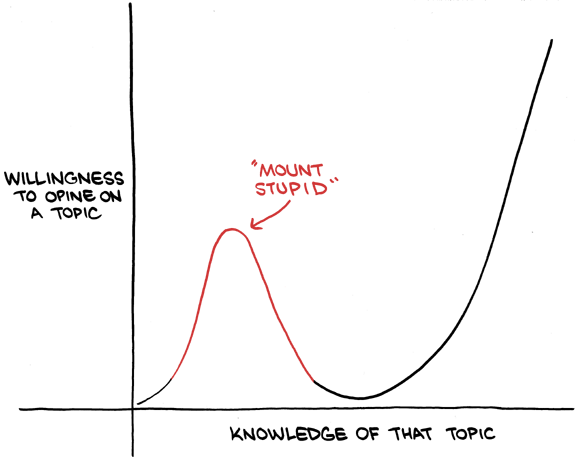
\includegraphics [scale=0.5]{Images/dunning_kruger.png} \\
%   {\small {\it \caption{Dunning–Kruger effect \label{fig:moun} \hcite{mount}}}}
% \end{figure}
    
% Conclusion
    \chapter{Conclusion}
    \textcolor{black}{As we have seen, the countdown to the 5G revolution has begun, and the explosion of connected devices, such as mobile phones, televisions, security systems and speakers, among others, is only going to intensify. As the next big thing in the journey of digital transformation, 5G will have an enormous impact on mankind. It will undoubtedly disrupt the way we live and work. It will go beyond mobile broadband and impact self-sustaining modern human establishments like smart cities, robotics and self-driving cars, and foster innovation in critical sectors such as health care, agriculture and education. Wearable devices and connected health care, for instance, will help people monitor and manage their illnesses and allow medical professionals to efficiently screen and diagnose patients remotely. In fact, the 5G network has the potential to enable surgeons to robotically operate on patients from thousands of miles away. This is possible because of the low-latency capabilities of 5G. With current networks, it takes approximately 100 milliseconds for information to travel across a network. This is incredibly fast, but there is still a lag that makes it impossible to communicate in real time. With 5G, that latency is expected to be reduced to 1 millisecond. Once you have the ability to communicate over a network in near real time, proximity will no longer matter. However, there are a lot of obstacles we need to overcome before a doctor in Los Angeles performs surgery on a patient in Boston.}

\section{A Long Road Ahead}
Obstacles such as cost and regulatory oversight will need to be resolved before the low-latency capabilities of 5G can open up a new world of possibilities. Communication service providers are going to need to invest billions of dollars in infrastructure to enable 5G. This includes investing in more antennas, base stations and fiber-optic cables, all of which must be in place before 5G can be widely adopted. It is safe to assume that, with all the hype around 5G, these providers will find a way to ultimately build the infrastructure needed, but it will take a significant amount of time and money before we will be able to rely on the 5G network completely. Additionally, governments and regulatory bodies will need to monitor advances and make it easier for telecommunication companies to invest in upgrading technology. They will need to enact policies to enable new revenue models, like data monetization and content management. Finally, once the initial obstacles have been hurdled, there will be new regulatory and liability considerations for advanced automated features such as remote surgery, remote health care, vehicle-to-vehicle communication and public safety.
\section{The Future of 5G}
2020 has been declared the year in which 5G will become commercially viable. Global carriers have started 5G speed trials, and there are promises of 5G-ready devices. As the world gears up for 5G implementation, translating the 5G promise into real impactful human experiences remains the challenge.
\item Developed cities will be the first to experience 5G, as rural areas currently lack the infrastructure to support the network, and it will take years before the whole world is connected. But even though we are just in the beginning stages of 5G, it is clearly not just a buzzword anymore. Companies are already having intense discussions around the massive implications of 5G on various industries and it will undoubtedly disrupt the way we live, work and play.\item In order to continue to advance technologically, however, we will need a stronger network. The future of innovation depends on the successful rollout and implementation of 5G — and when we get there, it will truly revolutionize the world

\section{What is 6G?}
\subsection{A Study of Next Generation Wireless Network}
Today the whole world is aware of the revolutionary changes in cell phone communication field. Wireless communication has brought in the new innovation in this field. In the context of the present scenario, the 3G experienced better internet. Later on, 3G has been improved. The urgency to have better communication networks than 5G has come which could be a completely wireless communication without any hindrance and limitations. It is completely advanced in terms of wireless communication. In the 5G system each and every cell phone will have a permanent home “IP address and care of address”.\item Now the awaiting future will experience 6G. In present time, cell phones have everything and are compact, with high memory and high speed with low power consumption. Today, Bluetooth technology and other technologies are like child’s play. 6G wireless cell phone communication network shall meet world class standard covering the whole world under its communication just like the Global covering system has been devised by some companies. This individual system creates difficulty in space roaming. The 7G mobile phone communication system is developed to integrate these in a one-unit communication system.

% \section{Future Research}

% \section{Chapter Summary}

    
% Bibliography
    \phantomsection
    \addcontentsline{toc}{chapter}{References}%
    \bibliography{bibliography}
    
    \vspace{2.0cm}
    \textcolor{black}{The 5G technology Argument \href{https://carrier.huawei.com/en/spotlight/5g}{referencing guidelines} in the Teaching and Learning platform. \url{https://carrier.huawei.com/en/spotlight/5g}}\\
  \item  Outlook: Visions and research directions for the Wireless World,
    WWRF, Oct 2011
    \item 5G Vision: The 5G Infrastructure Public Private Partnership: the next generation of
communication networks and services. From The 5G Infrastructure Public Private Partnership\href{https://5g-ppp.eu/wp-content/uploads/2015/02/5G-Vision-Brochure-v1.pdf}
    % Harvard referencing style '(Author, Year)'  and 'Author (Year)'
    % The template has an automated bibliography section based on references 
    % consistent with entries in the 'bibliography.bib' file 

% Appendices
    % \appendix
    % \chapter{(Appendix A title)}
    % \textcolor{red}{The final sections of your thesis are the appendices. Each appendix should be lettered (A, B, etc.,) and should consist of detailed information that is interesting but not essential to the main thrust of your findings section.\\
The appendices should be in the order that they are referred to in the main text. For instance, if Appendix A refers to something on page 25 and Appendix B refers to something on page 15, the appendices need to be re-lettered. This inconsistency occurs when text is moved around or inserted.)}

    
    %  \chapter{(Appendix B title)}
    % \input{Sections/Appendix_B}

\end{document}
%----------------------------------------------------------------------------------------------------%
